
The simulations carried out in this work consider the \ac{PL} varying uniformly across all users in the system with the channels drawn from the \textit{i.i.d.} samples. The queues are generated based on the Poisson process with the average values specified in each section presented. 
\begin{table*}
	\centering
	\caption{Sub-channel-wise listing of channel gains and rate allocations by different algorithms for a scheduling instant}
	\renewcommand{\arraystretch}{1.25} \scriptsize
	\begin{tabular}{|*{14}{c|}}
		\hline
		\multirow{2}{*}{Users} & \multirow{2}{*}{Queued} & \multicolumn{3}{c|}{\multirow{2}{*}{Channel Gains}} & \multicolumn{3}{c|}{Q-WSRME approach} & \multicolumn{3}{c|}{\multirow{2}{*}{JSFRA Scheme}} & \multicolumn{3}{c|}{Q-WSRM band} \\
		\multirow{2}{*}{} & \multirow{2}{*}{Packets} & \multicolumn{3}{c|}{} & \multicolumn{3}{c|}{(modified \review{\emph{backpressure}})} & \multicolumn{3}{c|}{} & \multicolumn{3}{c|}{Alloc Scheme} \\
		\cline{3-14}
		&& SC-\me{1} & SC-\me{2} & SC-\me{3} & SC-\me{1} & SC-\me{2} & SC-\me{3} & SC-\me{1} & SC-\me{2} & SC-\me{3} & SC-\me{1} & SC-\me{2} & SC-\me{3} \\
		\hline
		\me{1} & \me{4} & \me{1.71} &  \me{0.53}  &  \me{0.56} & \me{0} &  \me{0}  &  \me{0} & \me{4.0} &  \me{0}  &  \me{0} & \me{0} &  \me{0}  &  \me{0} \\
		\me{2} & \me{8} & \me{0.39} &  \me{1.41}  &  \me{1.03} & \me{0} &  \me{4.88}  &  \me{3.11} & \me{0} &  \me{5.49}  &  \me{0} & \me{0} &  \me{4.39}  &  \me{3.53} \\
		\me{3} & \me{4} & \me{2.34} &  \me{1.26}  &  \me{2.32} & \me{4.0} &  \me{0}  &  \me{0} & \me{0} &  \me{0}  &  \me{4.0} & \me{5.81} &  \me{0}  &  \me{0} \\
		\hline
		\multicolumn{5}{|c|}{Remaining backlogged packets (\me{\chi})} & \multicolumn{3}{c|}{\me{3.92} bits} & \multicolumn{3}{c|}{\me{2.51} bits} & \multicolumn{3}{c|}{\me{5.89} bits} \\
		\hline
	\end{tabular}
	\label{tbl-1}
\end{table*}
\begin{figure*}
	\centering
	\subfloat[][System Model \me{\lbrace N,N_B,K,N_T,N_R \rbrace = \lbrace 4,3,9,4,1\rbrace}]{
		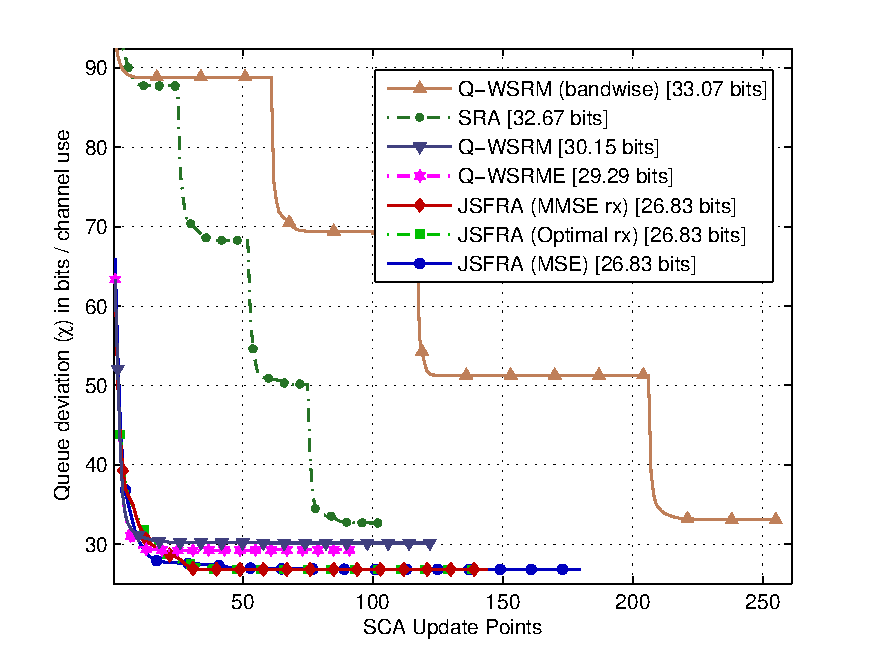
\includegraphics[width=0.5\textwidth]{fig-1-4}
		\label{fig-1}}
	\subfloat[][System Model \me{\lbrace N,N_B,K,N_T,N_R \rbrace = \lbrace 2,3,9,4,2\rbrace}]{
		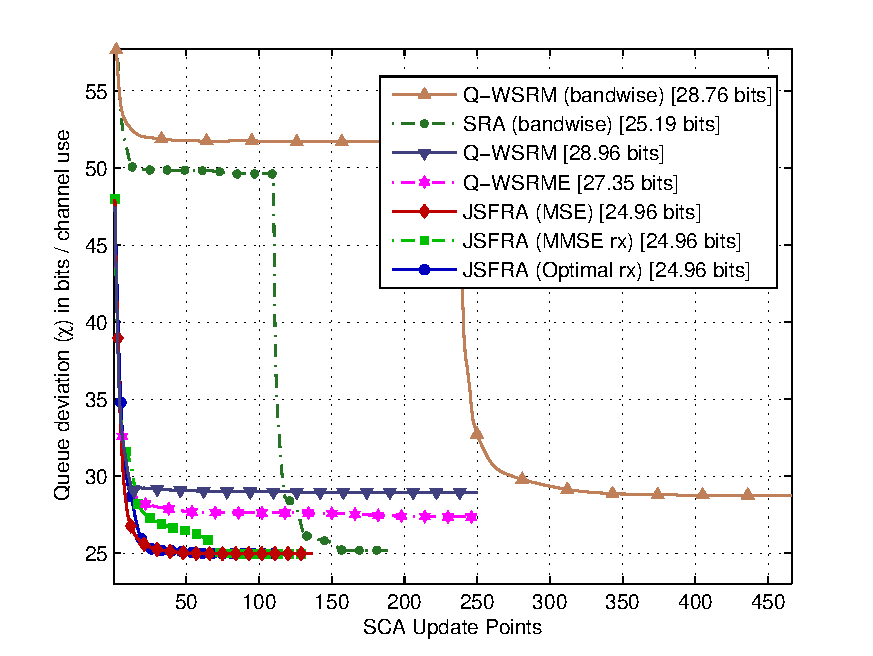
\includegraphics[width=0.5\textwidth]{fig-2-5}
		\label{fig-2}}
	\caption{Total number of backlogged packets \me{\chi} present in the system after each \ac{SCA} updates \review{using \me{\ell_1 (q = 1)} norm for \ac{JSFRA} schemes}}
	\label{fig-a}
\end{figure*}
